\chapter{Evaluation}
\label{cha:eval}

In this chapter, we present the case study. Section~\ref{sec:ch2_eval} describes the trace, the cache configurations and the cache sizes we compare. Section~\ref{sec:cache_behavior} analyzes how the cache behaves on this trace under prefix caching and under blending. In Section~\ref{sec:recommendation}, we use these results to decide when each mechanism should be used. Finally, Section~\ref{sec:ch1_eval} evaluates the accuracy of the agent frontend across several LLM backends.

\section{Setup}
\label{sec:ch2_eval}

We record the requests that the RepoGraph + Agentless frontend sends while working on SWE-bench issues, and replay them against vLLM with LMCache using the replay mechanism from Section~\ref{sec:request_logging}. Every configuration and cache size is run on the same trace.

\paragraph{Trace.}
We replay all prompts produced by RepoGraph + Agentless on SWE-bench Verified-mini \cite{MariusHobbhahn2025swe-bench-verified-mini}, which come from Django issues. The trace has 541 requests: 341 localization requests, 100 greedy repair requests, and 100 sampled repair requests, each of which asks for nine samples. Localization makes up 67\% of the prompt tokens in the trace, greedy repair 18\%, and sampled repair 15\%. We define the \emph{working set} of the trace as the KV cache that a cache of unlimited size would hold after the whole trace is replayed, with each distinct chunk (as blending splits the prompts) stored once. The working set has 4.1 million tokens. Each token takes 40\,KiB of KV cache on each GPU worker, so the working set is 157\,GiB per worker.

Figure~\ref{fig:length_dist} shows the distribution of request lengths. The median request has 5{,}042 tokens, half of the requests are between 1{,}792 and 6{,}978 tokens long, and a few requests reach up to 119{,}808 tokens.

\begin{figure}[H]
\centering
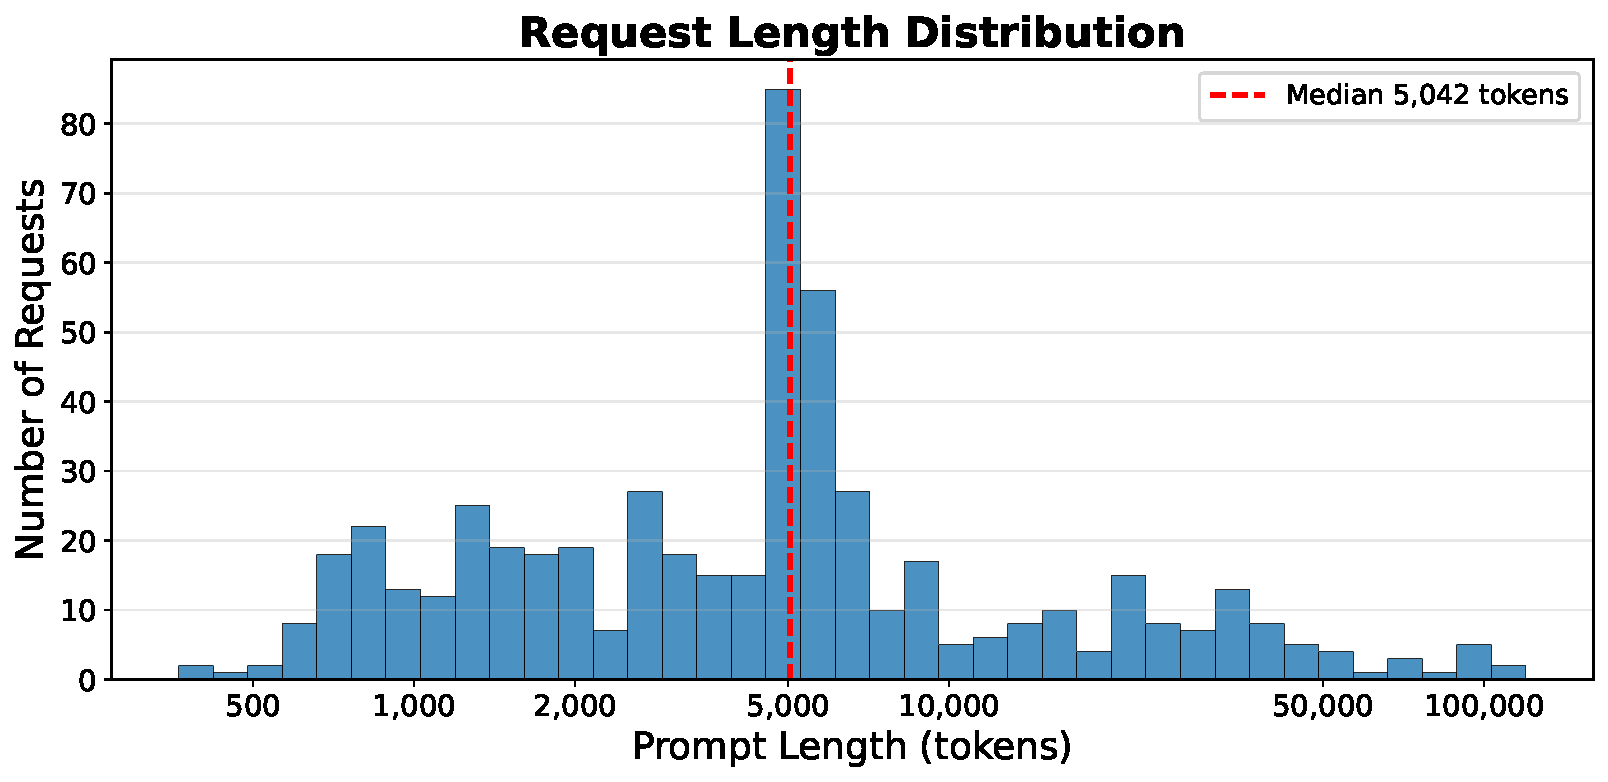
\includegraphics[width=0.7\linewidth]{graphs/case_study/length_distribution.pdf}
\vspace{-0.1in}
  \caption{\small Request length distribution of the trace ($n = 541$).}
 \label{fig:length_dist}
 \vspace{-0.15in}
\end{figure}

\paragraph{Model and hardware.}
We use Devstral Small in all experiments, which is also the open-source model in the accuracy evaluation (Section~\ref{sec:ch1_eval}). The model is served with 4-way tensor parallelism on four NVIDIA L40S GPUs.

\paragraph{Configurations.}
We compare two ways of reusing KV state across requests, both implemented in LMCache:
\begin{itemize}
    \item \textbf{Prefix caching} (baseline): KV state is reused in 1{,}024-token chunks, and only for chunks that match from the start of the prompt. This is the technique used by serving engines such as vLLM and SGLang.
    \item \textbf{Blend}: CacheBlend reuses any chunk of at least 256 tokens, wherever it appears in the prompt, and recomputes a fraction of the tokens (the \emph{recompute ratio}, set to 15\%) to repair the reused state.
\end{itemize}
In both configurations, we disable vLLM's own prefix cache, so KV state is only reused from LMCache's CPU cache. We run each configuration with five sizes of this cache per GPU worker: 1\%, 2\%, 5\% and 10\% of the working set (1.57, 3.14, 7.85 and 15.7\,GiB), and 40\,GiB, which holds a quarter of the working set.

\paragraph{Metrics.}
We use TTFT as our main latency metric. TTFT is the time from when a request arrives until the first output token is produced. It directly reflects the cost of the prefill phase, which is the phase that cache reuse speeds up. For a request that asks for several samples, TTFT is the time until the first token of the first sample. For each request, we define the \emph{TTFT speedup} as its TTFT under prefix caching divided by its TTFT under blending. A speedup above 1.0 means that blending made prefill faster, and a speedup below 1.0 means that it made prefill slower. To measure reuse, we use the \emph{cache hit ratio}, which is the fraction of prompt tokens loaded from the cache instead of recomputed, counted over all requests in the group we look at. Since the runs were spread over nodes with slightly different speeds, we normalize the TTFT of each run by its median ratio to a reference run, computed over the requests that no configuration hits.

\section{Cache Behavior}
\label{sec:cache_behavior}

In this section, we first look at which requests reuse cached state under each mechanism (Section~\ref{sec:cb_where}) and how this changes as the cache gets smaller (Section~\ref{sec:cb_size}). We then measure how much faster a request runs when blending reuses part of its prompt (Sections~\ref{sec:cb_worth} and~\ref{sec:cb_size_value}).

\subsection{Where the Reuse Comes From}
\label{sec:cb_where}

Figure~\ref{fig:hit_by_stage} shows the cache hit ratio at each cache size, broken down by the agent stage that sent the request.

\begin{figure}[H]
\centering
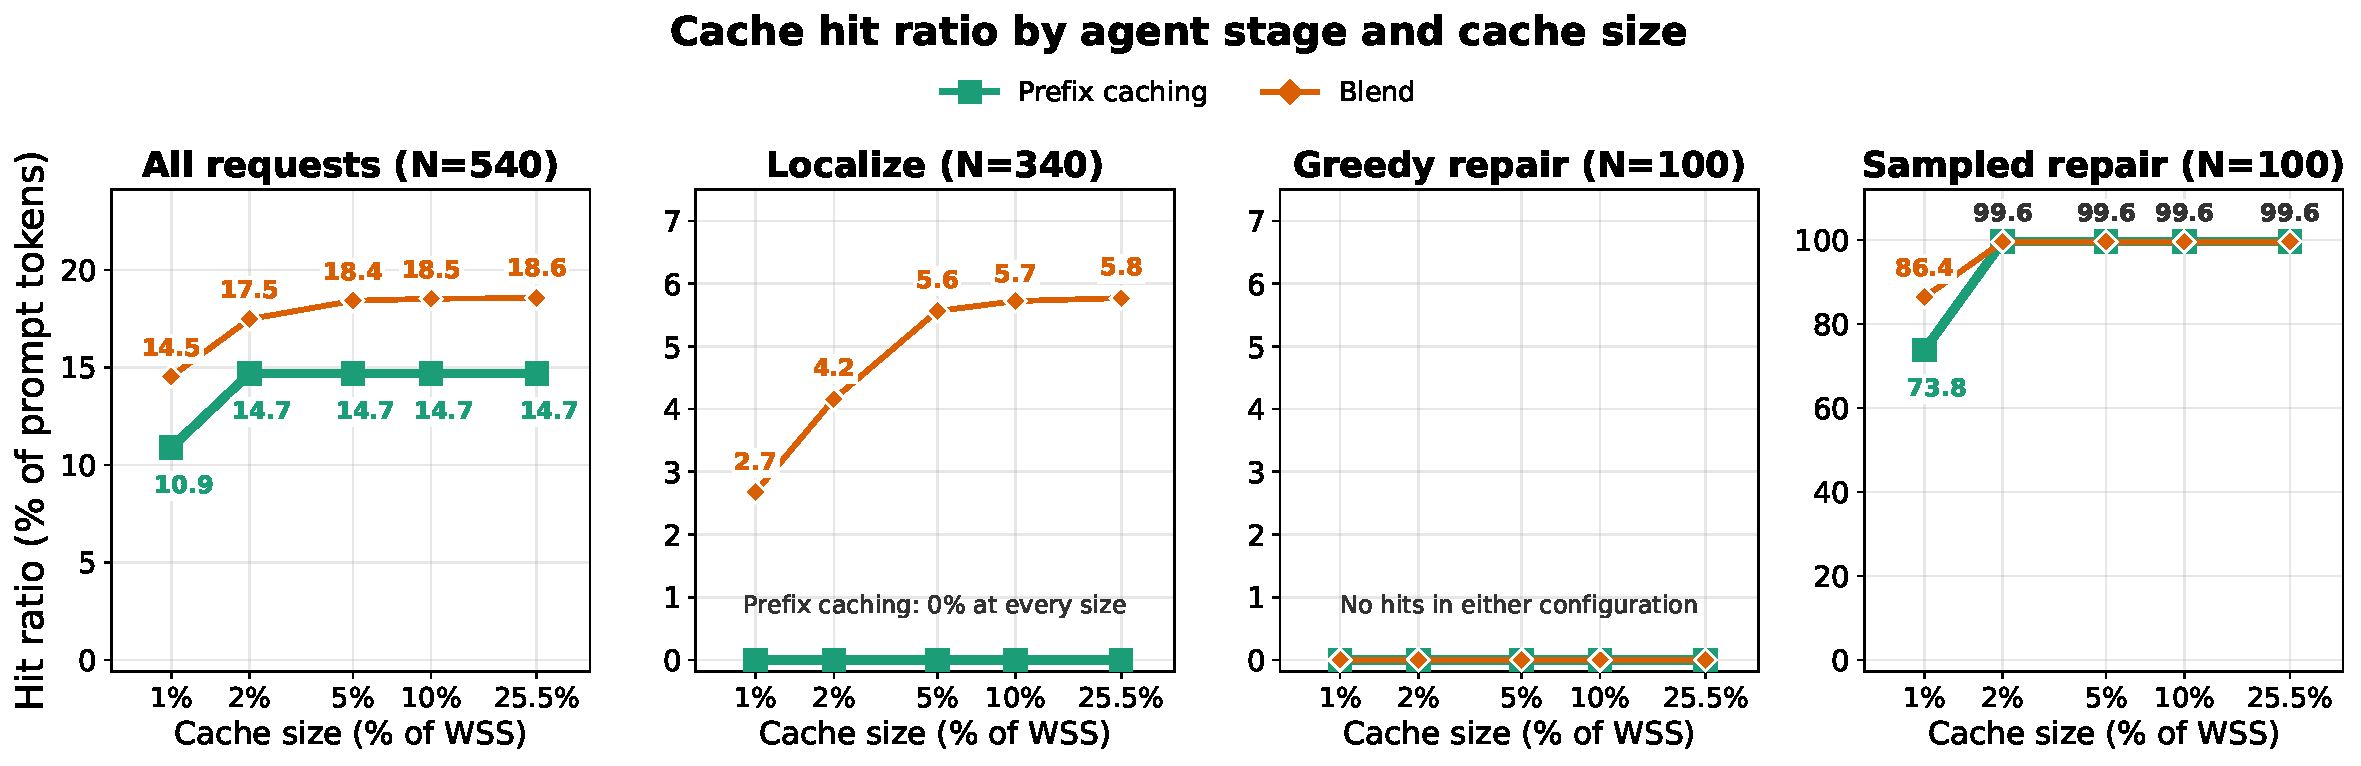
\includegraphics[width=\linewidth]{graphs/case_study/hit_ratio_by_stage_size.pdf}
\vspace{-0.1in}
  \caption{\small Cache hit ratio by agent stage and cache size, under prefix caching and blending.}
 \label{fig:hit_by_stage}
 \vspace{-0.15in}
\end{figure}

We find that most of the reuse in the trace comes from exact repeats. Each sampled repair request re-sends the greedy repair prompt right before it, so both mechanisms load 99.6\% of sampled repair tokens from the cache at every size from 2\% of the working set up. Sampled repair makes up 15\% of the prompt tokens in the trace, so these repeats explain almost all of prefix caching's 14.7\% hit ratio over the whole trace.

Blending adds reuse in only one stage, localization, which makes up two thirds of the prompt tokens in the trace. Prefix caching does not reuse any localization tokens. With the largest cache, blending loads 5.8\% of them from the cache, which raises the hit ratio over the whole trace from 14.7\% to 18.6\%. All localization hits follow the same pattern. The first few hundred tokens of the prompt, which contain the request's own issue text, miss in the cache, and the block of several thousand tokens that comes after them hits in full. Localization prompts for different issues share this block, but since it never appears at the start of the prompt, prefix caching cannot reuse it. This is the prompt layout we described in Section~\ref{sec:design_cc}.

Greedy repair requests do not share any reusable content with earlier requests, so neither mechanism gets hits on them.

\subsection{Cache Size}
\label{sec:cb_size}

Figure~\ref{fig:hit_vs_size} shows how the hit ratio over the whole trace changes with cache size, from 1\% of the working set up to 40\,GiB (a quarter of the working set). Exact repeats and blending's extra hits react to a smaller cache in very different ways.

\begin{figure}[H]
\centering
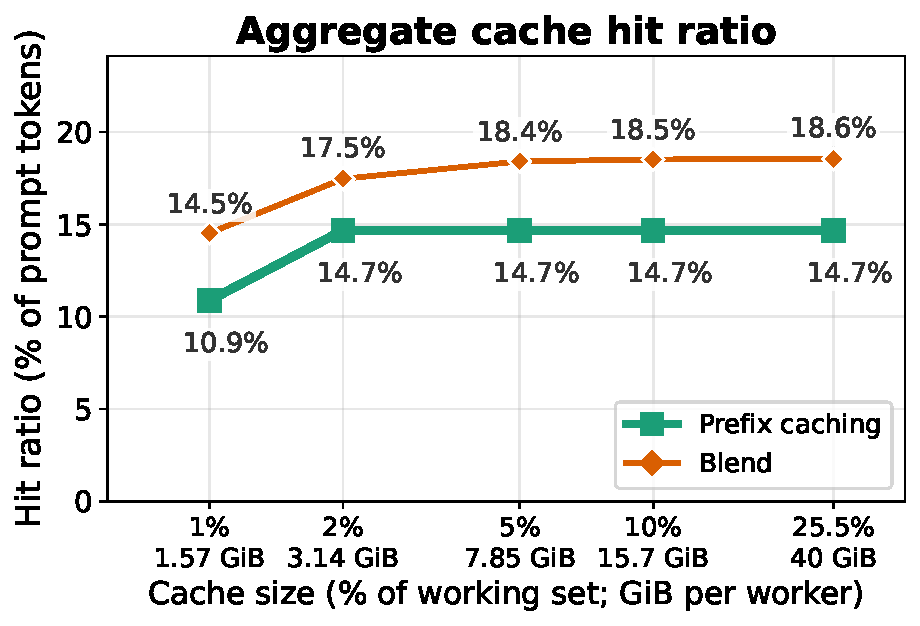
\includegraphics[width=0.6\linewidth]{graphs/case_study/hit_ratio_vs_cache_size.pdf}
\vspace{-0.1in}
  \caption{\small Trace-wide cache hit ratio against cache size, under prefix caching and blending.}
 \label{fig:hit_vs_size}
 \vspace{-0.15in}
\end{figure}

An exact repeat is reused by the very next request, so it stays in the cache even when the cache is small. As a result, prefix caching's hit ratio stays at 14.7\% at every size from 2\% of the working set up to 40\,GiB. Blending's extra hits, on the other hand, come from localization prompts that are reused long after they are stored, after many other requests have gone through the cache. These entries are therefore the first to be evicted when the cache shrinks. Blending's hit ratio is 14.5\% at 1\% of the working set and 17.5\% at 2\%, and stays between 18.4\% and 18.6\% from 5\% up. Out of the 45 localization requests that blending hits at some cache size, only 18 still hit at 1\%.

At 1\% of the working set, prefix caching starts to lose some of its exact repeats as well, and its hit ratio drops to 10.9\%. This is because LMCache evicts the oldest chunks of a prompt first, which are the chunks at the start of the prompt. Since prefix caching has to match a prompt from its first chunk, a repeat whose first chunks have been evicted cannot be reused at all. Blending looks up each chunk separately and can still reuse the chunks that remain in the cache. At 1\%, it loads 86\% of sampled repair tokens from the cache, compared to 74\% for prefix caching. As a result, blending's advantage over prefix caching is 3.6 percentage points at 1\% of the working set, drops to 2.8 points at 2\%, and rises again to 3.7 points at 5\%.

\subsection{What a Hit Is Worth}
\label{sec:cb_worth}

So far we have looked at how often blending hits. We now look at how much a hit speeds up a request. Figure~\ref{fig:speedup_delta} plots the TTFT speedup of blending over prefix caching for each localization and greedy repair request, with a cache size of 5\% of the working set. The x-axis is the request's hit-ratio gain $\delta$, which is the fraction of its prompt that blending loads from the cache minus the fraction that prefix caching loads. Since prefix caching does not hit any of these requests, $\delta$ is equal to blending's hit ratio.

\begin{figure}[H]
\centering
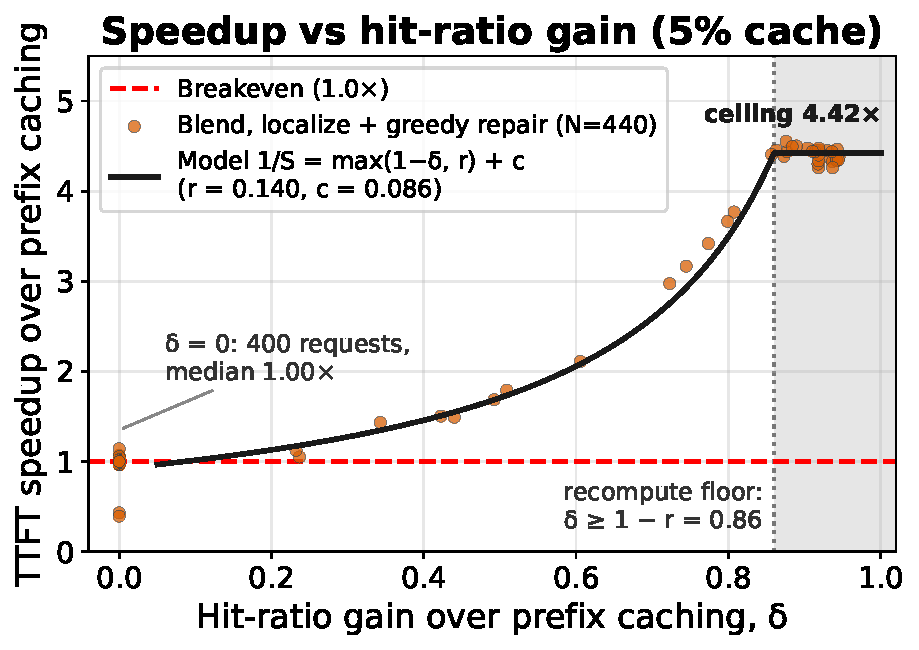
\includegraphics[width=0.6\linewidth]{graphs/case_study/speedup_vs_delta_5pct.pdf}
\vspace{-0.1in}
  \caption{\small TTFT speedup of blending over prefix caching against hit-ratio gain $\delta$, for localization and greedy repair requests at a cache size of 5\% of the working set, with the cost model of Equation~\ref{eq:blend_cost}.}
 \label{fig:speedup_delta}
 \vspace{-0.15in}
\end{figure}

The 400 requests that blending does not hit run at the same speed as under prefix caching (median 1.00$\times$). For the 40 requests that it hits, the speedup first increases with $\delta$ and then flattens out, with a median of 4.35$\times$. This shape comes from how blending repairs the reused state. Blending recomputes every token that it could not reuse. If these tokens make up less than a fixed fraction $r$ of the prompt (the recompute ratio), it also recomputes tokens selected from the reused chunks until it reaches $r$. Each blend also has a fixed cost $c$ for loading and processing the cached state. Relative to computing the whole prompt from scratch, the cost of a request is therefore
\begin{equation}
\label{eq:blend_cost}
\frac{1}{S(\delta)} = \max(1-\delta,\ r) + c,
\end{equation}
where $S$ is the speedup. Fitting this model to the 40 hits gives $r = 0.14$, which is close to the configured recompute ratio of 0.15, and $c = 0.086$. When $\delta$ is larger than $1-r$, blending still has to recompute a fraction $r$ of the prompt, so reusing more of the prompt no longer reduces the cost. The speedup is then capped at $1/(r+c) \approx 4.4\times$, and 26 of the 40 hits are on this plateau. In other words, for most localization hits the speedup is limited by the recompute ratio rather than by how much of the prompt is reused.

\subsection{What Cache Size Changes}
\label{sec:cb_size_value}

Figure~\ref{fig:speedup_delta_grid} shows the same comparison for the localization requests at every cache size. Figure~\ref{fig:localize_paired} tracks the 45 localization requests that blending hits at some cache size across all five sizes.

\begin{figure}[H]
\centering
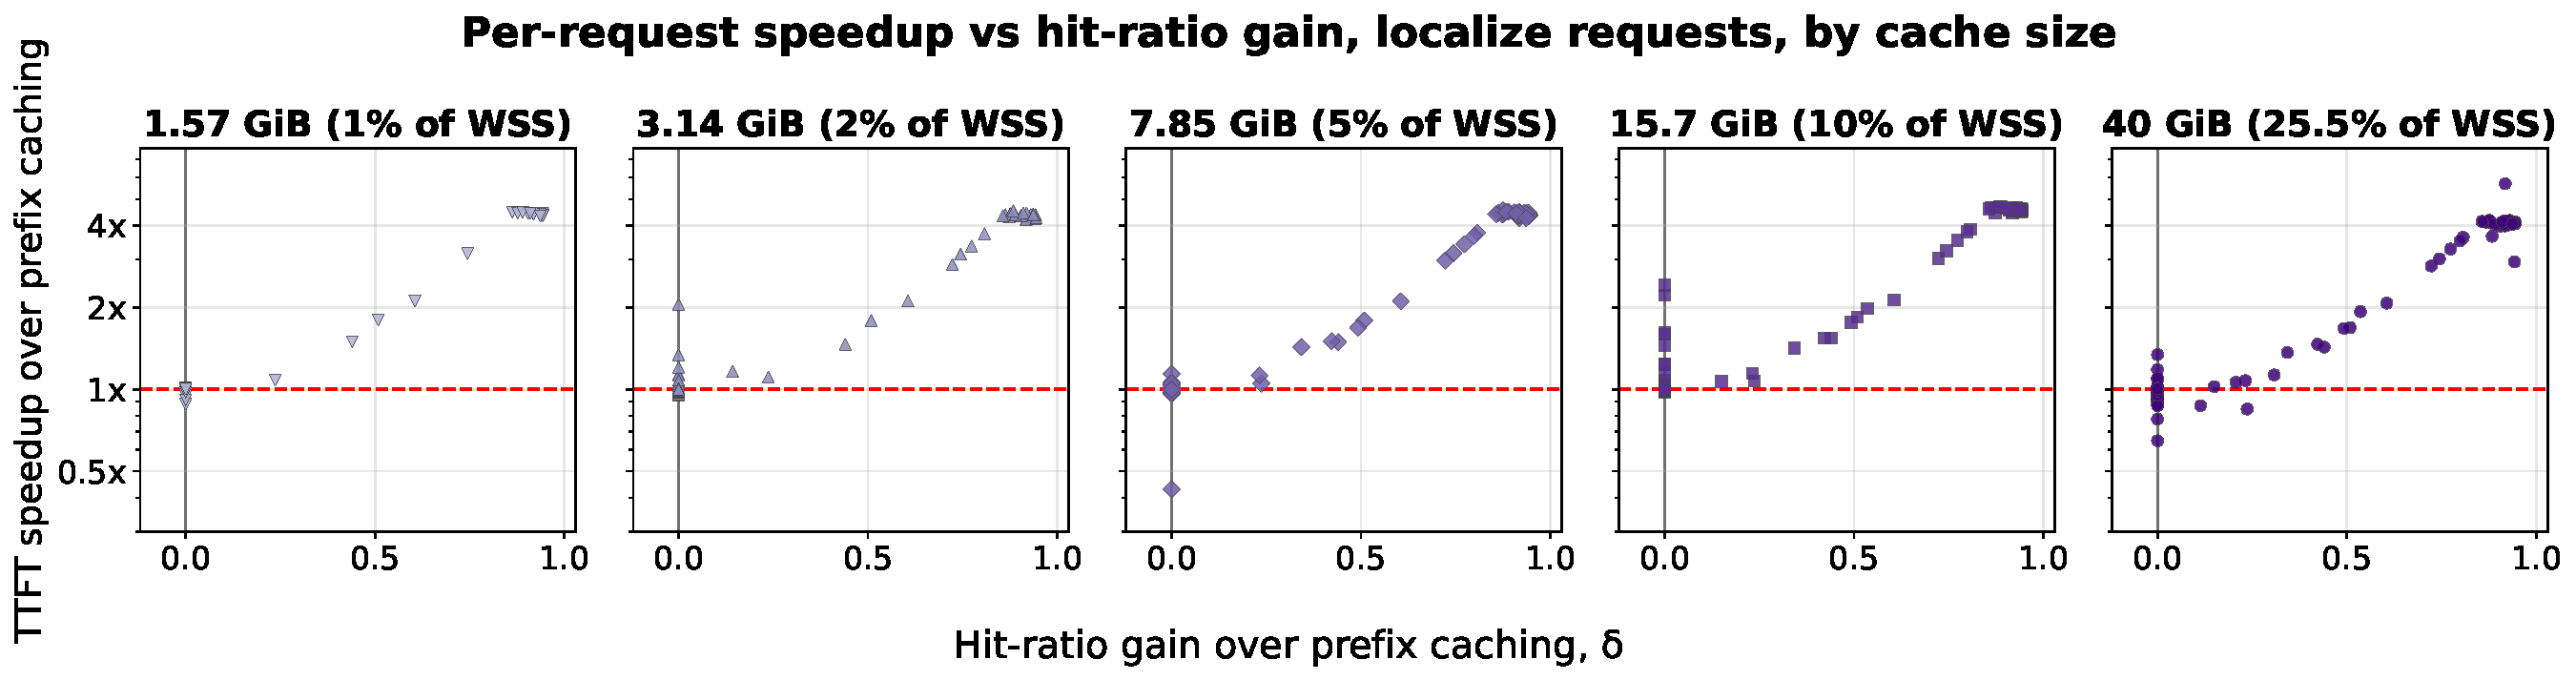
\includegraphics[width=\linewidth]{graphs/case_study/speedup_vs_delta_grid_prefix.pdf}
\vspace{-0.1in}
  \caption{\small TTFT speedup of blending over prefix caching against hit-ratio gain, for localization requests, at each cache size.}
 \label{fig:speedup_delta_grid}
 \vspace{-0.15in}
\end{figure}

\begin{figure}[H]
\centering
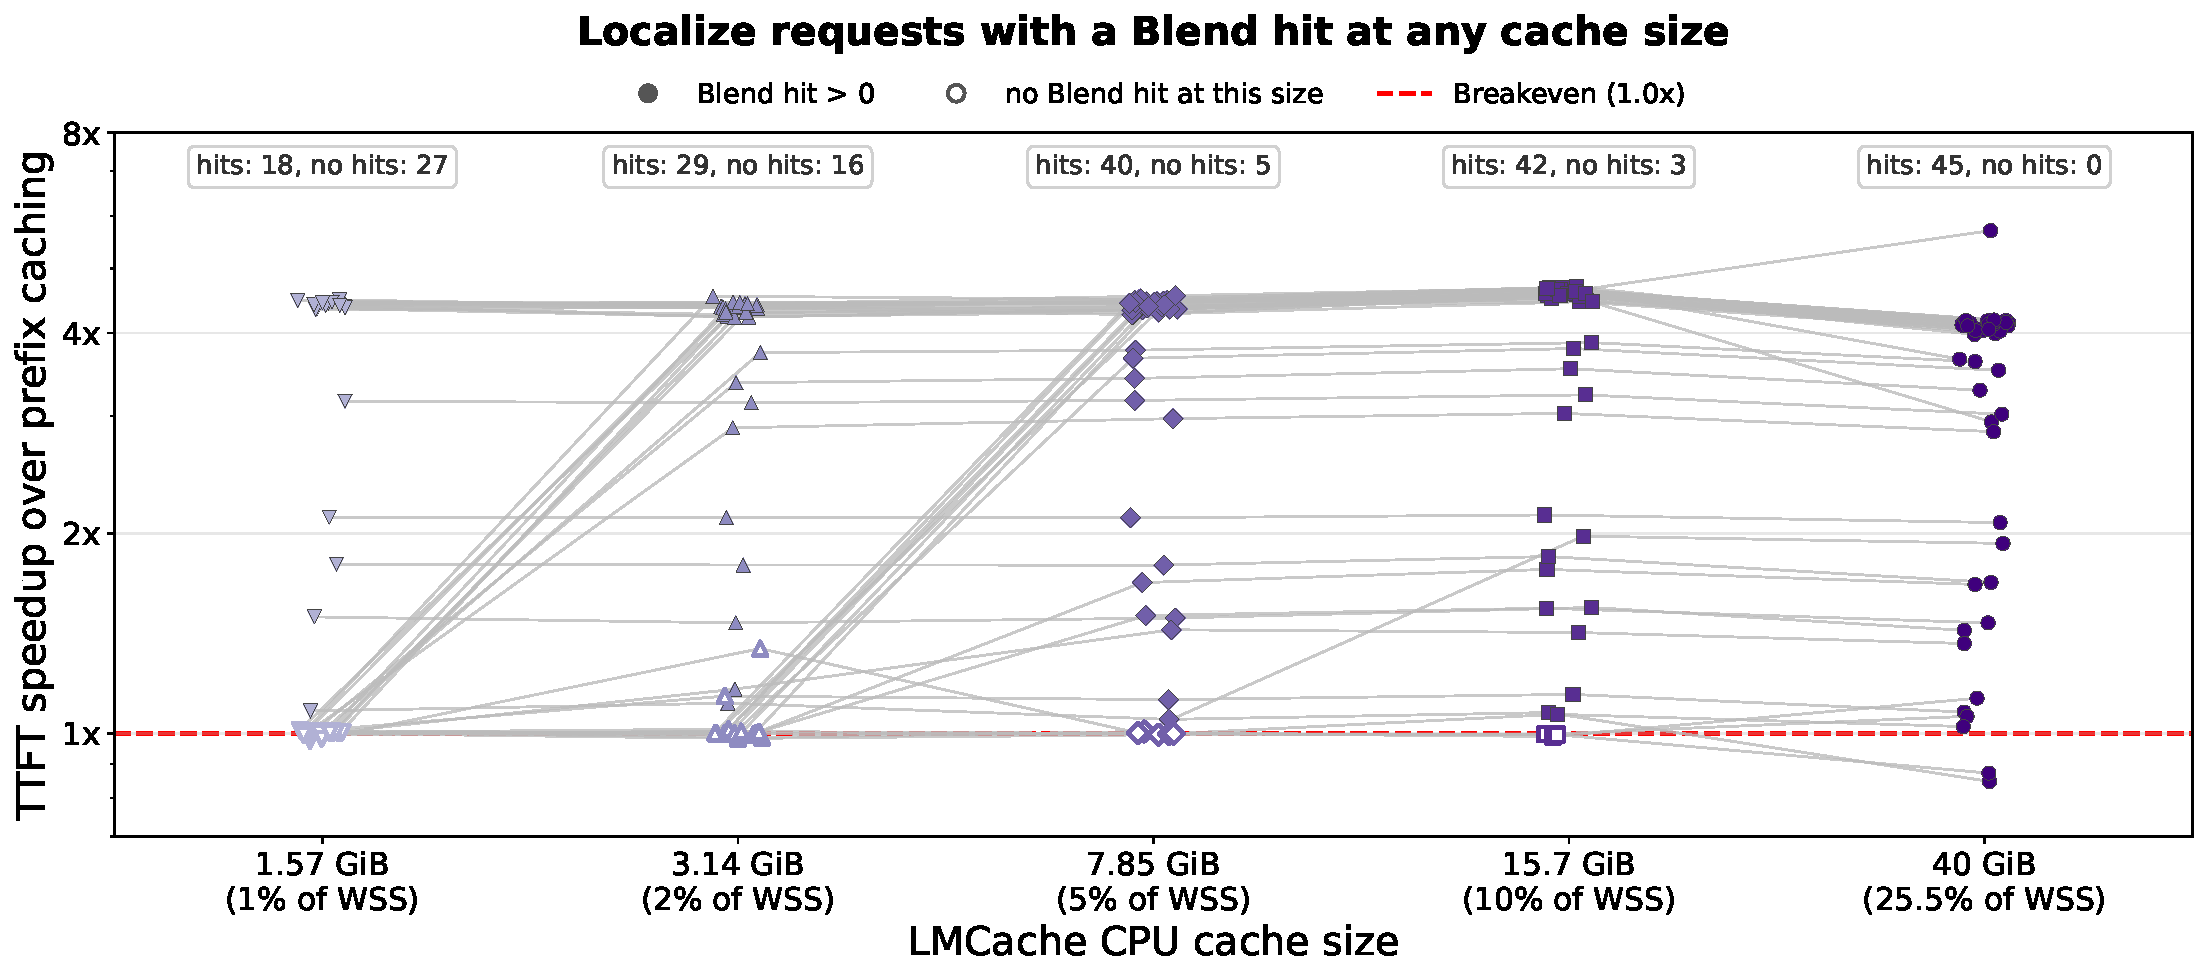
\includegraphics[width=\linewidth]{graphs/case_study/localize_hit_paired_prefix.pdf}
\vspace{-0.1in}
  \caption{\small The 45 localization requests that blending hits at some cache size, followed across cache sizes. Hollow markers have no blending hit at that size.}
 \label{fig:localize_paired}
 \vspace{-0.15in}
\end{figure}

The speedup curve looks the same at every cache size. The median speedup of the requests that blending hits stays between 4.0$\times$ and 4.6$\times$ from 1\% of the working set up to 40\,GiB. What changes with a smaller cache is the number of requests that hit. Of the 45 localization requests, 18 hit at 1\% of the working set, 29 at 2\%, 40 at 5\%, 42 at 10\%, and all 45 at 40\,GiB. A request that loses its hit is not slower than under prefix caching. It simply runs at prefix-caching speed, with a median speedup of 1.00$\times$ at every size. So as the cache shrinks, blending loses its gains gradually, one request at a time, but the requests that lose their hits do not get any slower.

\subsection{Beyond Django}
\label{sec:cb_other_repos}

The trace we study comes from a single repository. How much reuse blending can find depends on the workload, for example on how often the agent's tasks share repository context, how long that context is, and how far apart in time the tasks that share it arrive. To study other repositories without serving their traces, we built a simulator that replays a trace through the cache's lookup and eviction policy. The simulator reproduces the measured hit ratios of both mechanisms at every cache size from 2\% of the working set upward.

\mytodo{Run the simulator on agent traces from repositories larger and smaller than Django. Report how the gap between blending and prefix caching, and its sensitivity to cache size, vary with the workload, and whether repository size or another factor (for example, how often tasks share a base commit, or the prompt layout) decides when blending has more to reuse.}

\subsection{Case Study: Routing Requests Around the Cache}
\label{sec:recommendation}

The results above establish that only 17.7\% of requests in our trace are faster under blending, and that whether a request wins is governed by its cache hit ratio rather than its size. This raises a practical design question: since the cache path is not universally profitable, can a request be routed \emph{before} it reaches LMCache, so that requests unlikely to benefit go straight to vanilla vLLM? This subsection is a case study of that question: it examines what a routing controller would need to decide, and what the measured data says each candidate decision rule is actually worth. The question is worth asking precisely because cache reuse costs nothing in output quality, as Section~\ref{sec:ch1_eval} goes on to show, which leaves latency as the only axis on which the routing decision has to be made.

\subsubsection{Is There a Prompt-Length Floor?}
\label{sec:rec_length_floor}

The natural first rule is a prompt-length floor. The intuition is that the cache path carries a startup cost that a short prompt cannot amortize, so below some length the lookup cannot pay for itself even in the best case. The data offers only partial support for this intuition, and establishing what support there is requires care about how prompt length is measured.

Testing it requires per-request token counts taken from the serving log rather than inferred from latency. The distinction matters: speedup is itself a ratio of baseline latency, so inferring prompt length from that same baseline would make length and speedup share a term and manufacture a correlation between them. Against measured token counts the correlation between length and speedup among well-cached requests is $r = -0.001$, whereas inferring length from baseline latency yields $r = +0.63$. All lengths reported here are measured.

Figure~\ref{fig:crossover} plots median TTFT speedup against prompt length, separately for requests that hit the cache (hit ratio above 70\%) and requests that effectively miss it (hit ratio below 5\%). Prompts under 1{,}000 tokens are excluded, because at that size the cache path takes a near-constant 0.16\,s and the speedup ratio is set by how the vanilla baseline happened to be scheduled rather than by prompt size.

Among the requests that hit, prompt length separates two regimes. Between 1{,}000 and 3{,}000 tokens they sit below breakeven, with a median of 0.80$\times$ in the lower bucket and 0.62$\times$ in the upper, and fewer than half beating the baseline. Beyond 4{,}500 tokens they sit well above it, at a median of 2.10$\times$ with 98\% beating the baseline. The median crosses breakeven once, at roughly 2{,}967 tokens, within an interval of 2{,}659 to 4{,}183 tokens that reflects how coarsely the region is sampled.

That sampling is the main caveat on the crossing. Of the 85 well-cached requests at or above 1{,}000 tokens, 64 fall in a narrow band between 4{,}837 and 5{,}811 tokens, and only four lie between 2{,}000 and 4{,}500. The curve therefore interpolates across the region where the crossing occurs rather than measuring through it, and it is comparing two fairly distinct populations of requests rather than tracking one population as it grows. The single well-cached request above 9{,}000 tokens scores 0.57$\times$, which points the other way, though one request settles nothing. We therefore treat the crossing as evidence that a length effect exists among well-cached requests, not as a precise threshold.

The bucket below 1{,}000 tokens is an exception that is best read as noise rather than signal. Its median speedup is 1.66$\times$, but individual values run from 0.17$\times$ to 9.24$\times$. At these sizes the blend path takes a near-constant ${\sim}$0.16\,s, so the ratio is governed entirely by how the vanilla baseline happened to be scheduled, and six of the nineteen requests in that bucket record a baseline above 0.4\,s, which is far more than a sub-1{,}000-token prefill should cost. We therefore do not treat that bucket as evidence for or against a floor.

\begin{figure}[H]
\centering
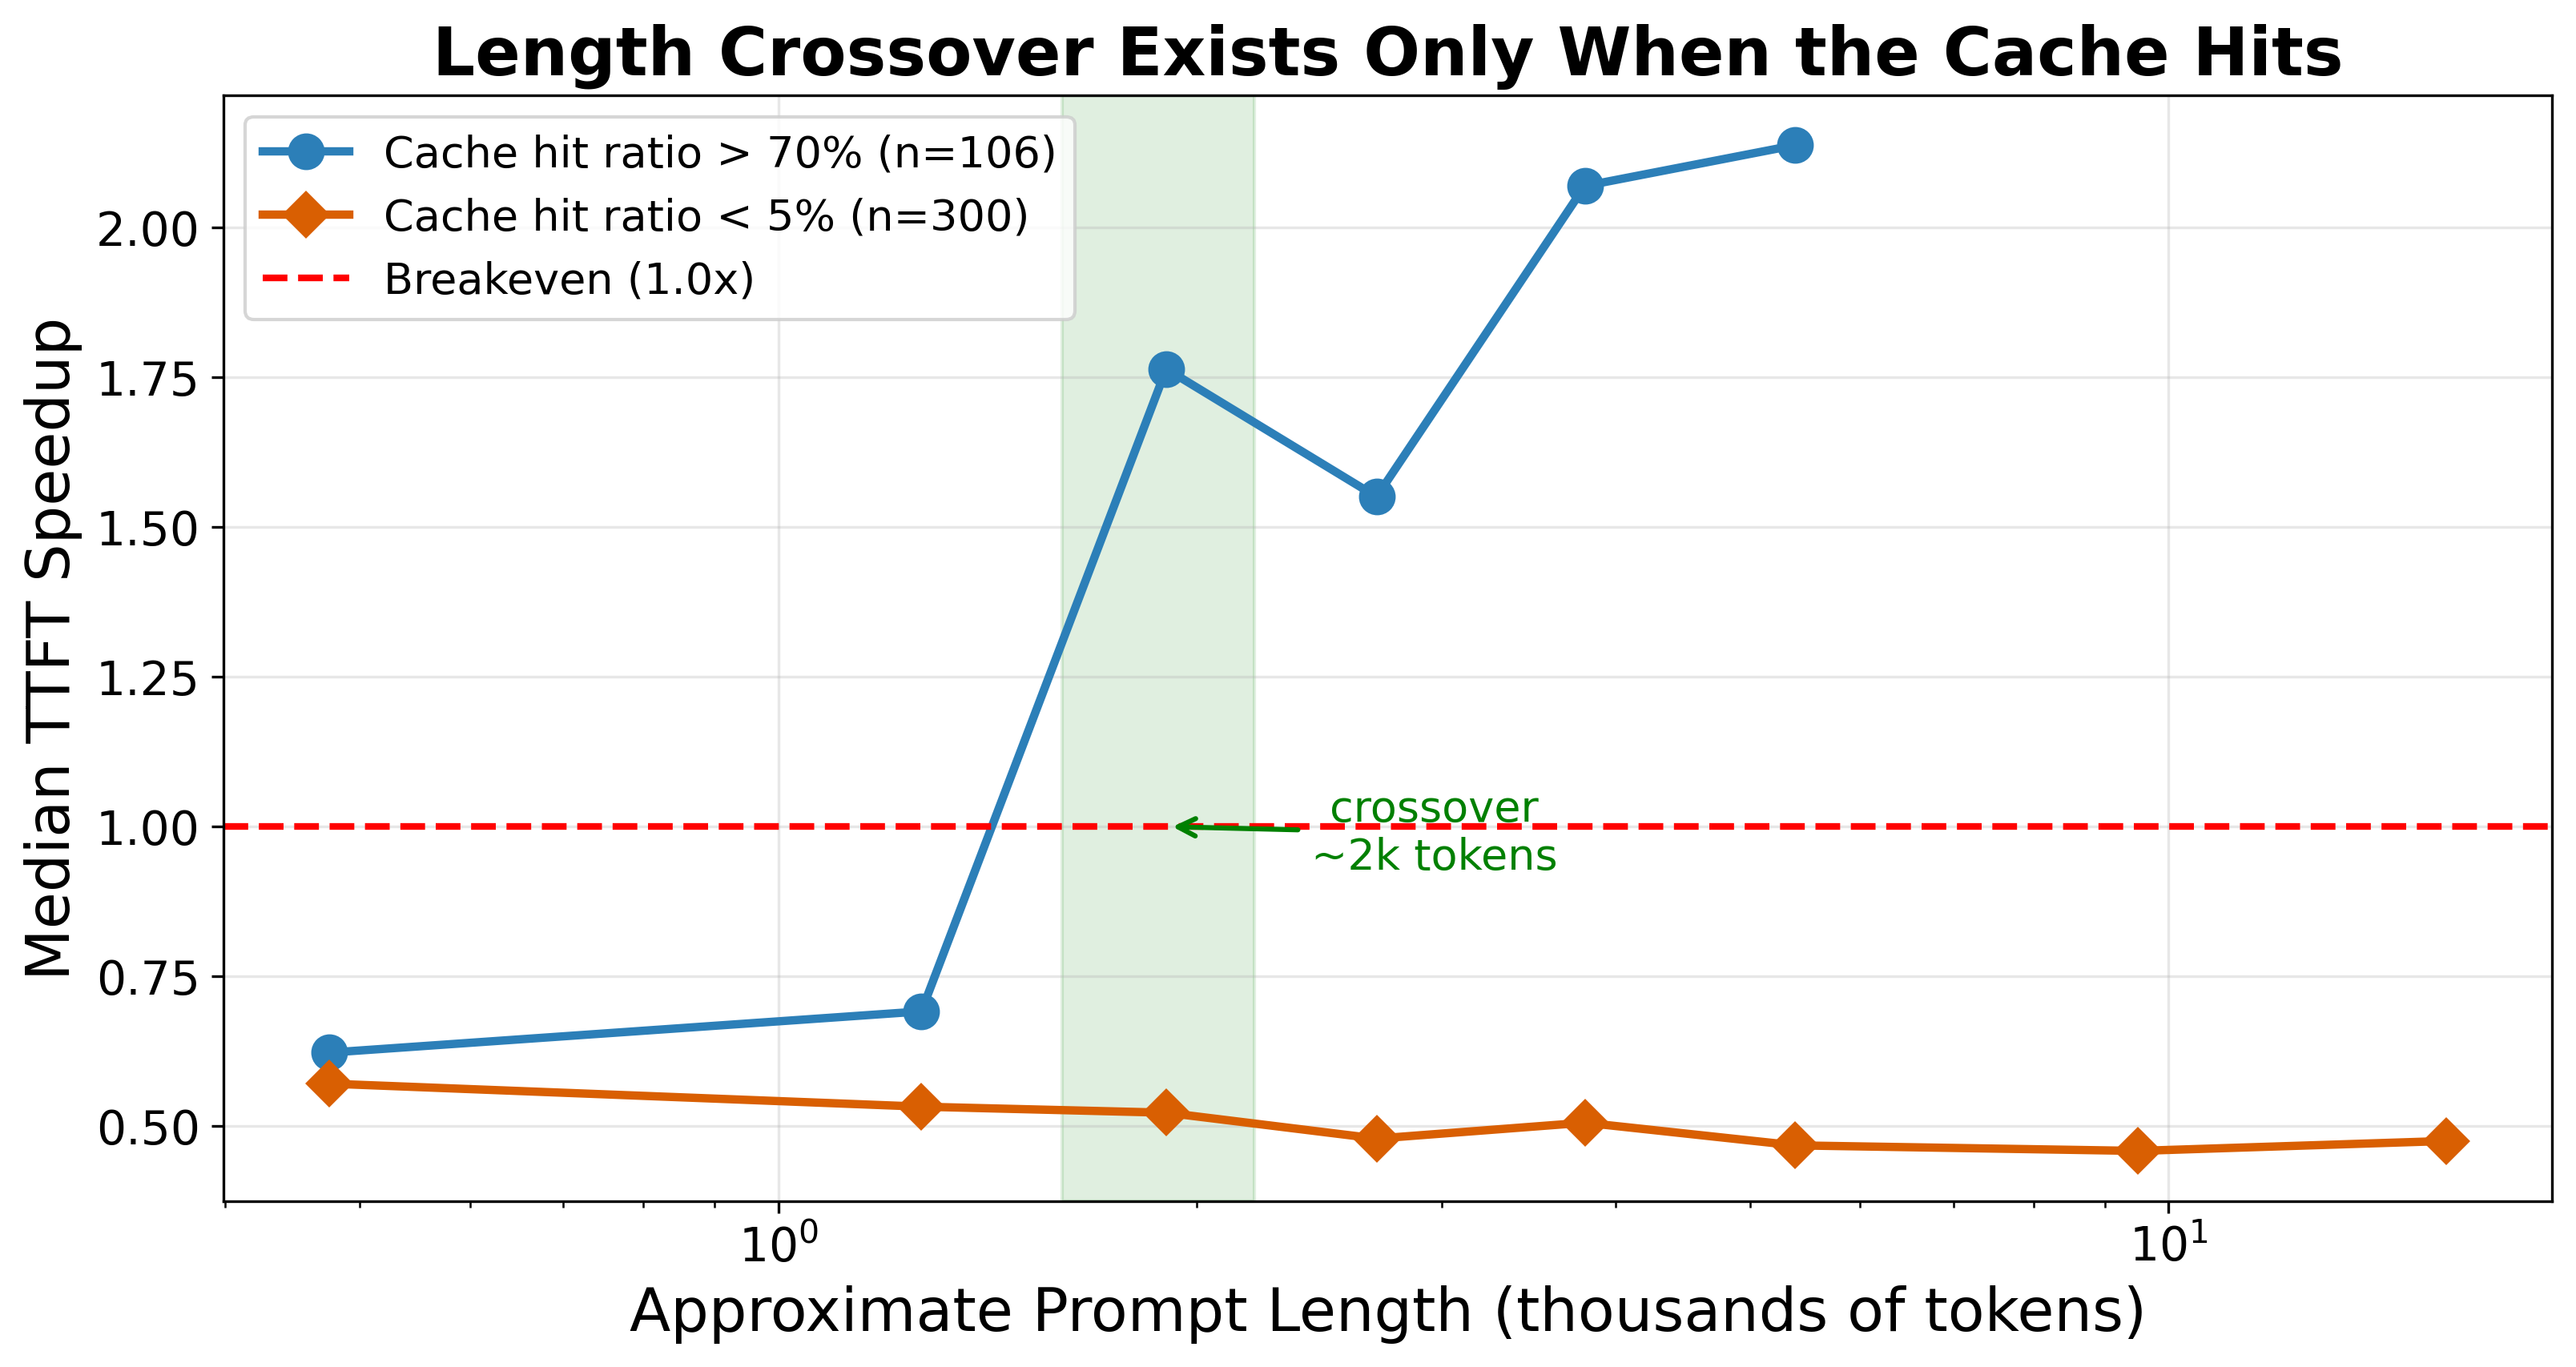
\includegraphics[width=0.9\linewidth]{graphs/thesis_variance_figures/crossover_by_hit_cluster.png}
\vspace{-0.1in}
  \caption{\small Median TTFT speedup vs.\ prompt length, split by cache hit ratio. Requests that hit the cache sit below breakeven from 1{,}000 to 3{,}000 tokens and well above it beyond 4{,}500; the shaded band marks the interval containing the single crossing. Requests that miss sit near $0.5\times$ at every length, so no length threshold recovers them. Prompts under 1{,}000 tokens are excluded because the cache path's fixed cost dominates the ratio at that size.}
 \label{fig:crossover}
 \vspace{-0.15in}
\end{figure}

For the requests that miss, the picture is entirely different. Their median speedup is 0.46--0.57$\times$ in every length bucket from under 1{,}000 tokens to over 12{,}000 tokens, and essentially none beat the baseline at any length. The penalty for a cache miss is close to scale-invariant: enabling LMCache roughly doubles TTFT whether the prompt is short or long. A length floor therefore cannot help this population, because there is no length at which they stop losing.

This exposes the limitation of the rule. A length floor is only useful to the extent that length predicts whether a request will hit. Figure~\ref{fig:length_vs_hits} plots the two against each other, using the measured token counts and the same served-run hit ratios as Figure~\ref{fig:speedup_3d}. The two clusters and the empty band between them appear here as well, which is the point: hit ratio is close to binary on this workload, and the question is whether length tells us which side a request will land on. It does so only weakly, at $r = -0.21$. The median hit ratio declines with length, from 20\% below 1{,}000 tokens to 2.6\% in the 6{,}000 to 10{,}000 range and 0.4\% above 30{,}000, but well-cached requests appear at every length. Knowing a prompt's length narrows the odds without determining the outcome.

\begin{figure}[H]
\centering
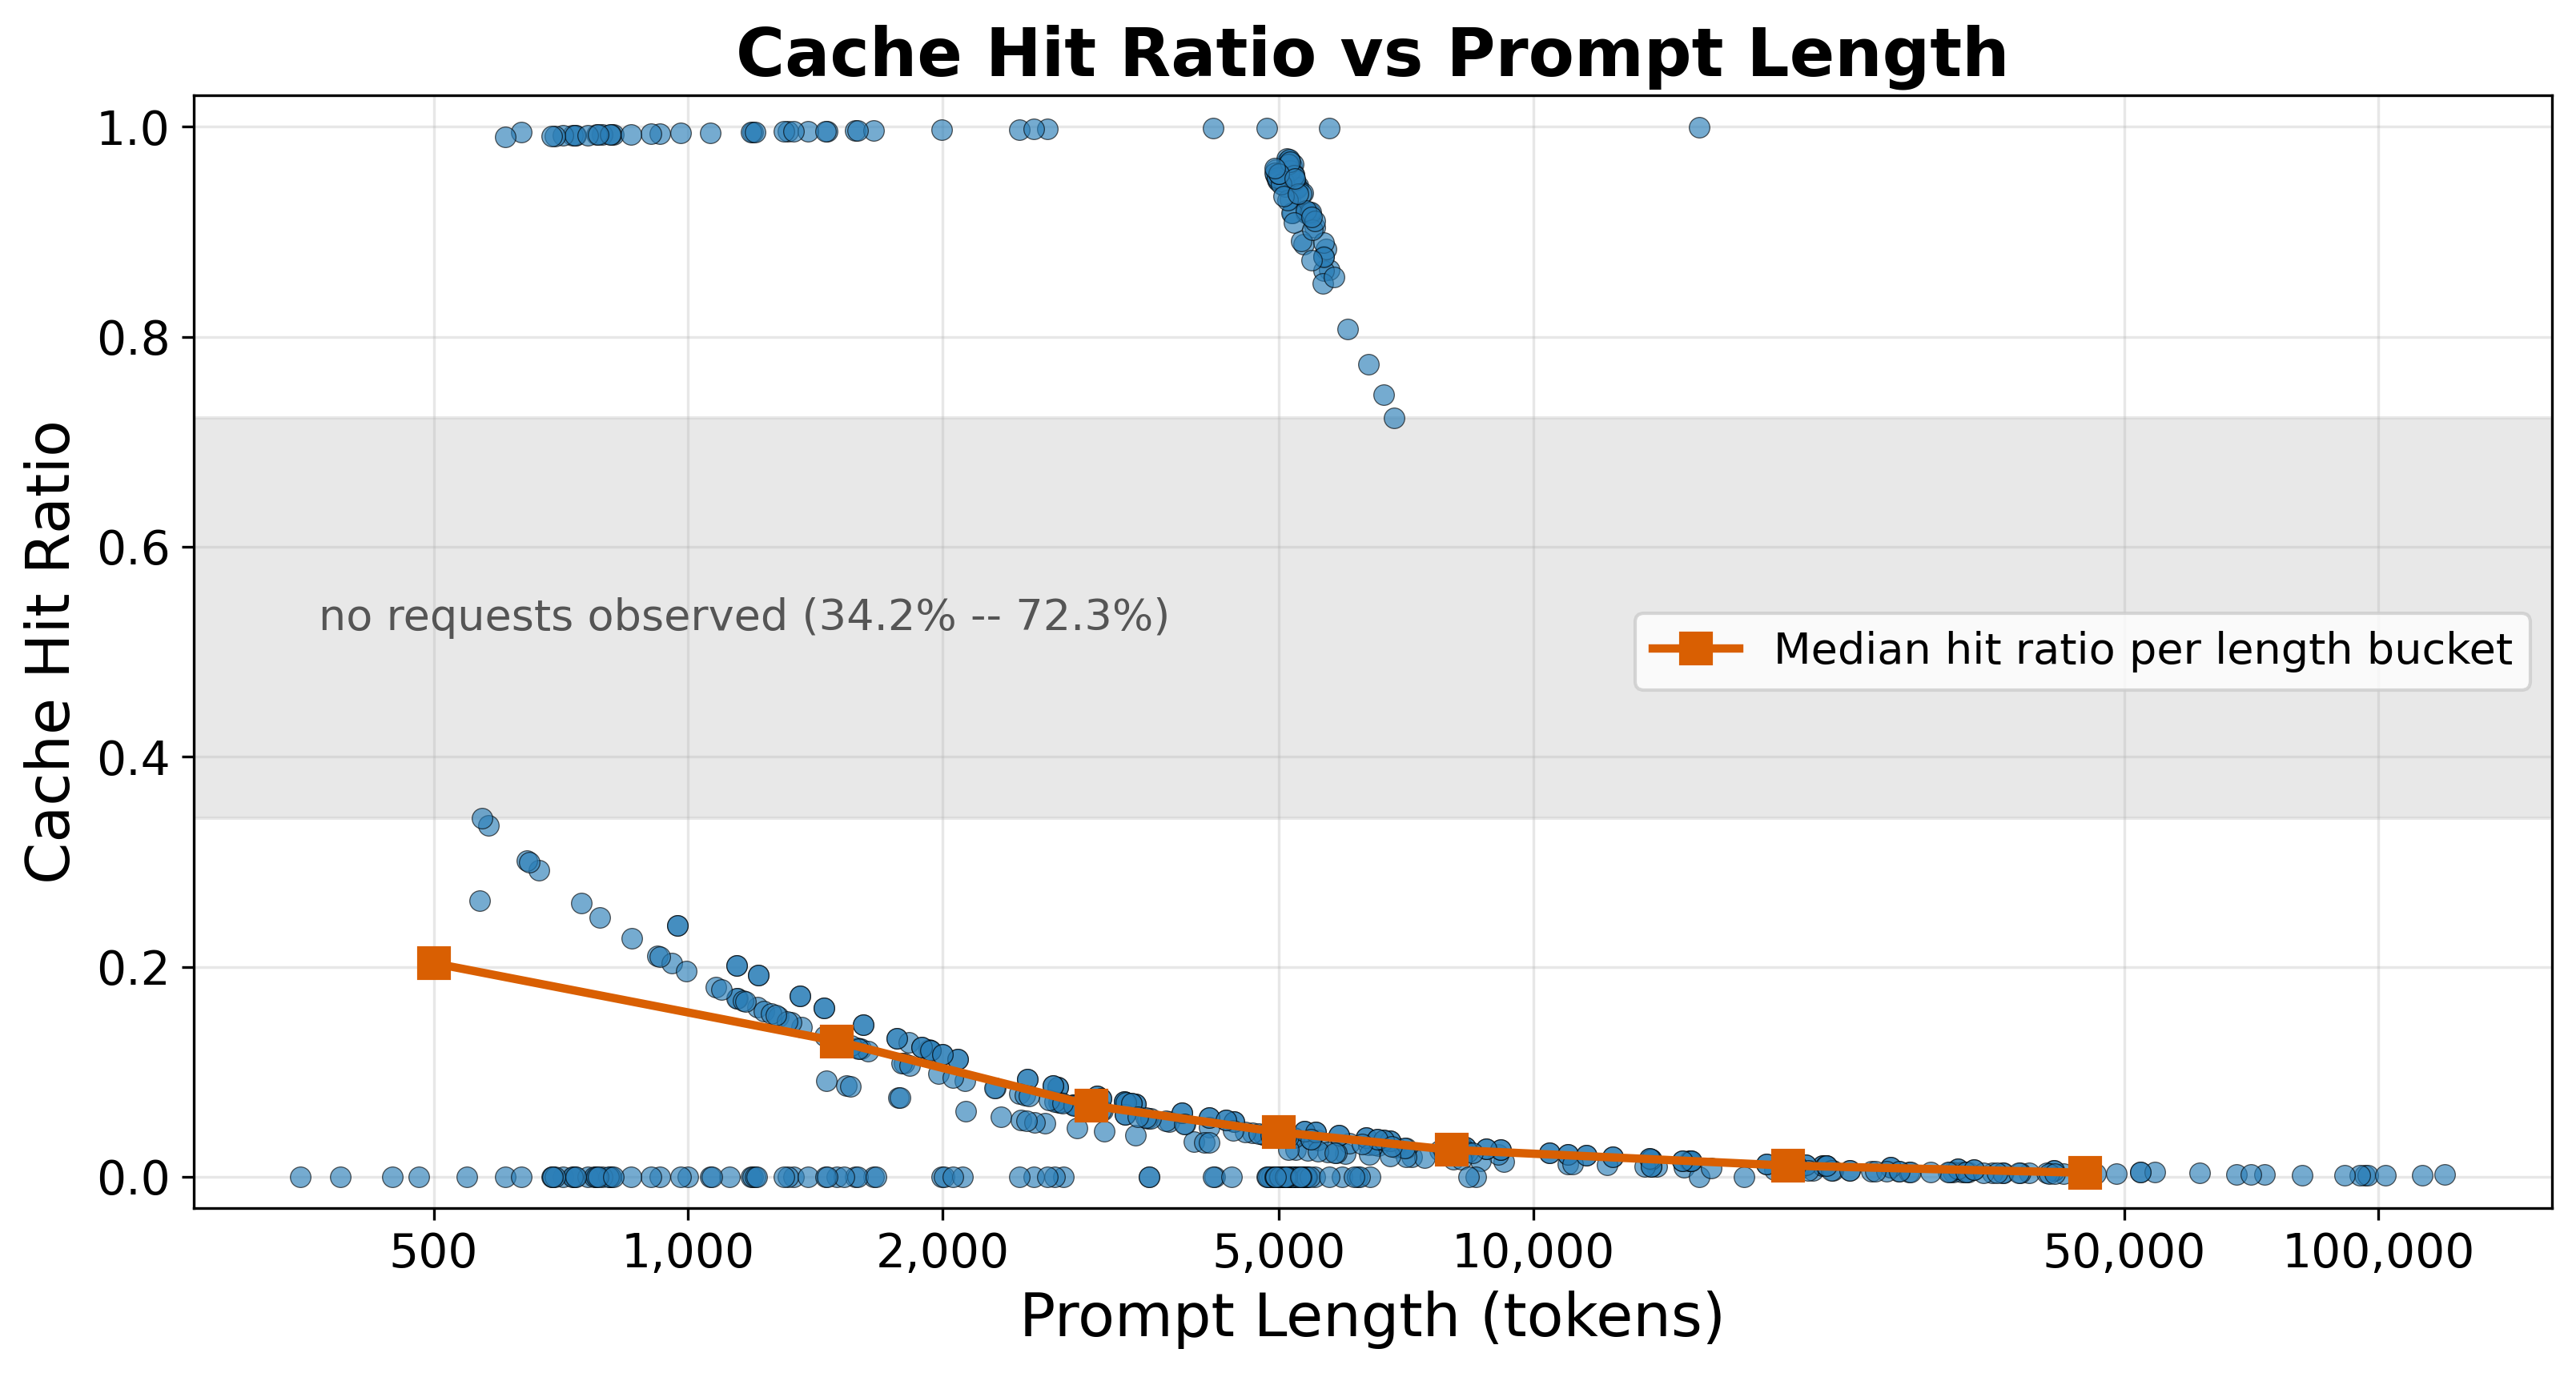
\includegraphics[width=0.85\linewidth]{graphs/thesis_variance_figures/length_vs_hitratio.png}
\vspace{-0.1in}
  \caption{\small Served-run cache hit ratio against measured prompt length ($n = 536$). The same two clusters and the same empty band appear as in Figure~\ref{fig:speedup_3d}. Length is a weak predictor of which cluster a request falls into ($r = -0.21$): the per-bucket median declines with length, but well-cached requests occur at every length.}
 \label{fig:length_vs_hits}
 \vspace{-0.15in}
\end{figure}

The declining median is what the upper gate in Section~\ref{sec:rec_gate_effect} exploits. Beyond 6{,}000 tokens the median hit ratio falls to 2.6\% and keeps dropping, reaching 0.4\% above 30{,}000, so bypassing the long tail gives up little reuse. This is a property of how this agent assembles long prompts rather than of the caching mechanism, and it would need rechecking on a workload whose long requests overlap more.

\subsubsection{Why the Miss Penalty Does Not Shrink With Length}
\label{sec:rec_miss_penalty}

The scale invariance follows from where the cost is incurred. On a miss, the retrieve path finds nothing and vLLM performs its normal prefill, so the lookup itself is cheap. The expense is on the \emph{store} side. The connector's \texttt{wait\_for\_save} runs the entire GPU-to-CPU offload of the newly computed KV synchronously, and vLLM calls it inside \texttt{execute\_model} before logits are computed and before the sampler runs. The offloaded volume is exactly linear in the number of stored tokens. Every byte of that transfer therefore lands inside TTFT, and it grows in proportion to the prompt, which is why the ratio rather than the absolute penalty is what stays constant.

This is a consequential observation for the controller design, because it means the miss penalty is not an intrinsic property of position-independent reuse. It is a property of storing synchronously on the critical path. Moving the offload to a background stream, so that a request pays only for what it reads and not for what it writes, would remove the penalty for the 80\% of our trace that misses. We did not implement this change, and validating it is the highest-value next step identified by this evaluation.

\subsubsection{What Length-Based Routing Actually Buys}
\label{sec:rec_gate_effect}

The crossover suggests a floor. In aggregate, however, the floor is not the rule that matters. Figure~\ref{fig:gated_hist} compares three policies on the same trace: routing everything through the cache, applying a 2{,}000-token floor, and applying a band that adds an upper threshold at 6{,}000 tokens. We measure each by the aggregate deficit, the extra wall-clock time the cache path costs across the whole trace relative to serving every request on vanilla vLLM. Serving the entire trace on vanilla vLLM takes 726\,s of TTFT in total, which is the reference point for these figures.

Routing everything through LMCache costs 772\,s more than that. A 2{,}000-token floor barely moves it, to 748\,s, even though it bypasses 149 of 536 requests. It recovers 3\% of the deficit while giving up 28\% of the traffic. Raising the floor does not rescue it either: a 5{,}000-token floor still leaves 698\,s while bypassing half the workload. The reason is visible in the figure. The sub-breakeven mode is populated at every length, so removing short requests removes about as much benefit as cost, and the median speedup of what remains falls slightly rather than rising.

The upper threshold is what pays. An upper gate alone at 6{,}000 tokens, with no floor at all, brings the deficit from 772\,s to 101\,s. That single rule accounts for 87\% of the total recovery available from any length-based policy we swept. Adding the 2{,}000-token floor on top brings it to 78\,s. The mechanism is the one identified above: long prompts in this trace rarely hit, so they pay the full synchronous store cost with almost no compensating read. The upper gate is therefore better understood as a crude reuse gate than as a length gate. It works because length correlates with reuse at the top of this range, not because length is the quantity that matters.

Two properties of this result are worth noting. The recovery comes from removing large absolute losses rather than from improving the typical request: the median speedup of the routed population stays near 0.51$\times$ under every policy we swept, while the aggregate improves by an order of magnitude. And the remaining deficit is small but not zero. The narrowest band, 5{,}000 to 6{,}000 tokens, brings it to 27\,s while routing 111 of 536 requests, which is close to bracketing this workload's dominant prompt size; the wider 2{,}000 to 6{,}000 band is the more general rule at a deficit of 78\,s.

\begin{figure}[H]
\centering
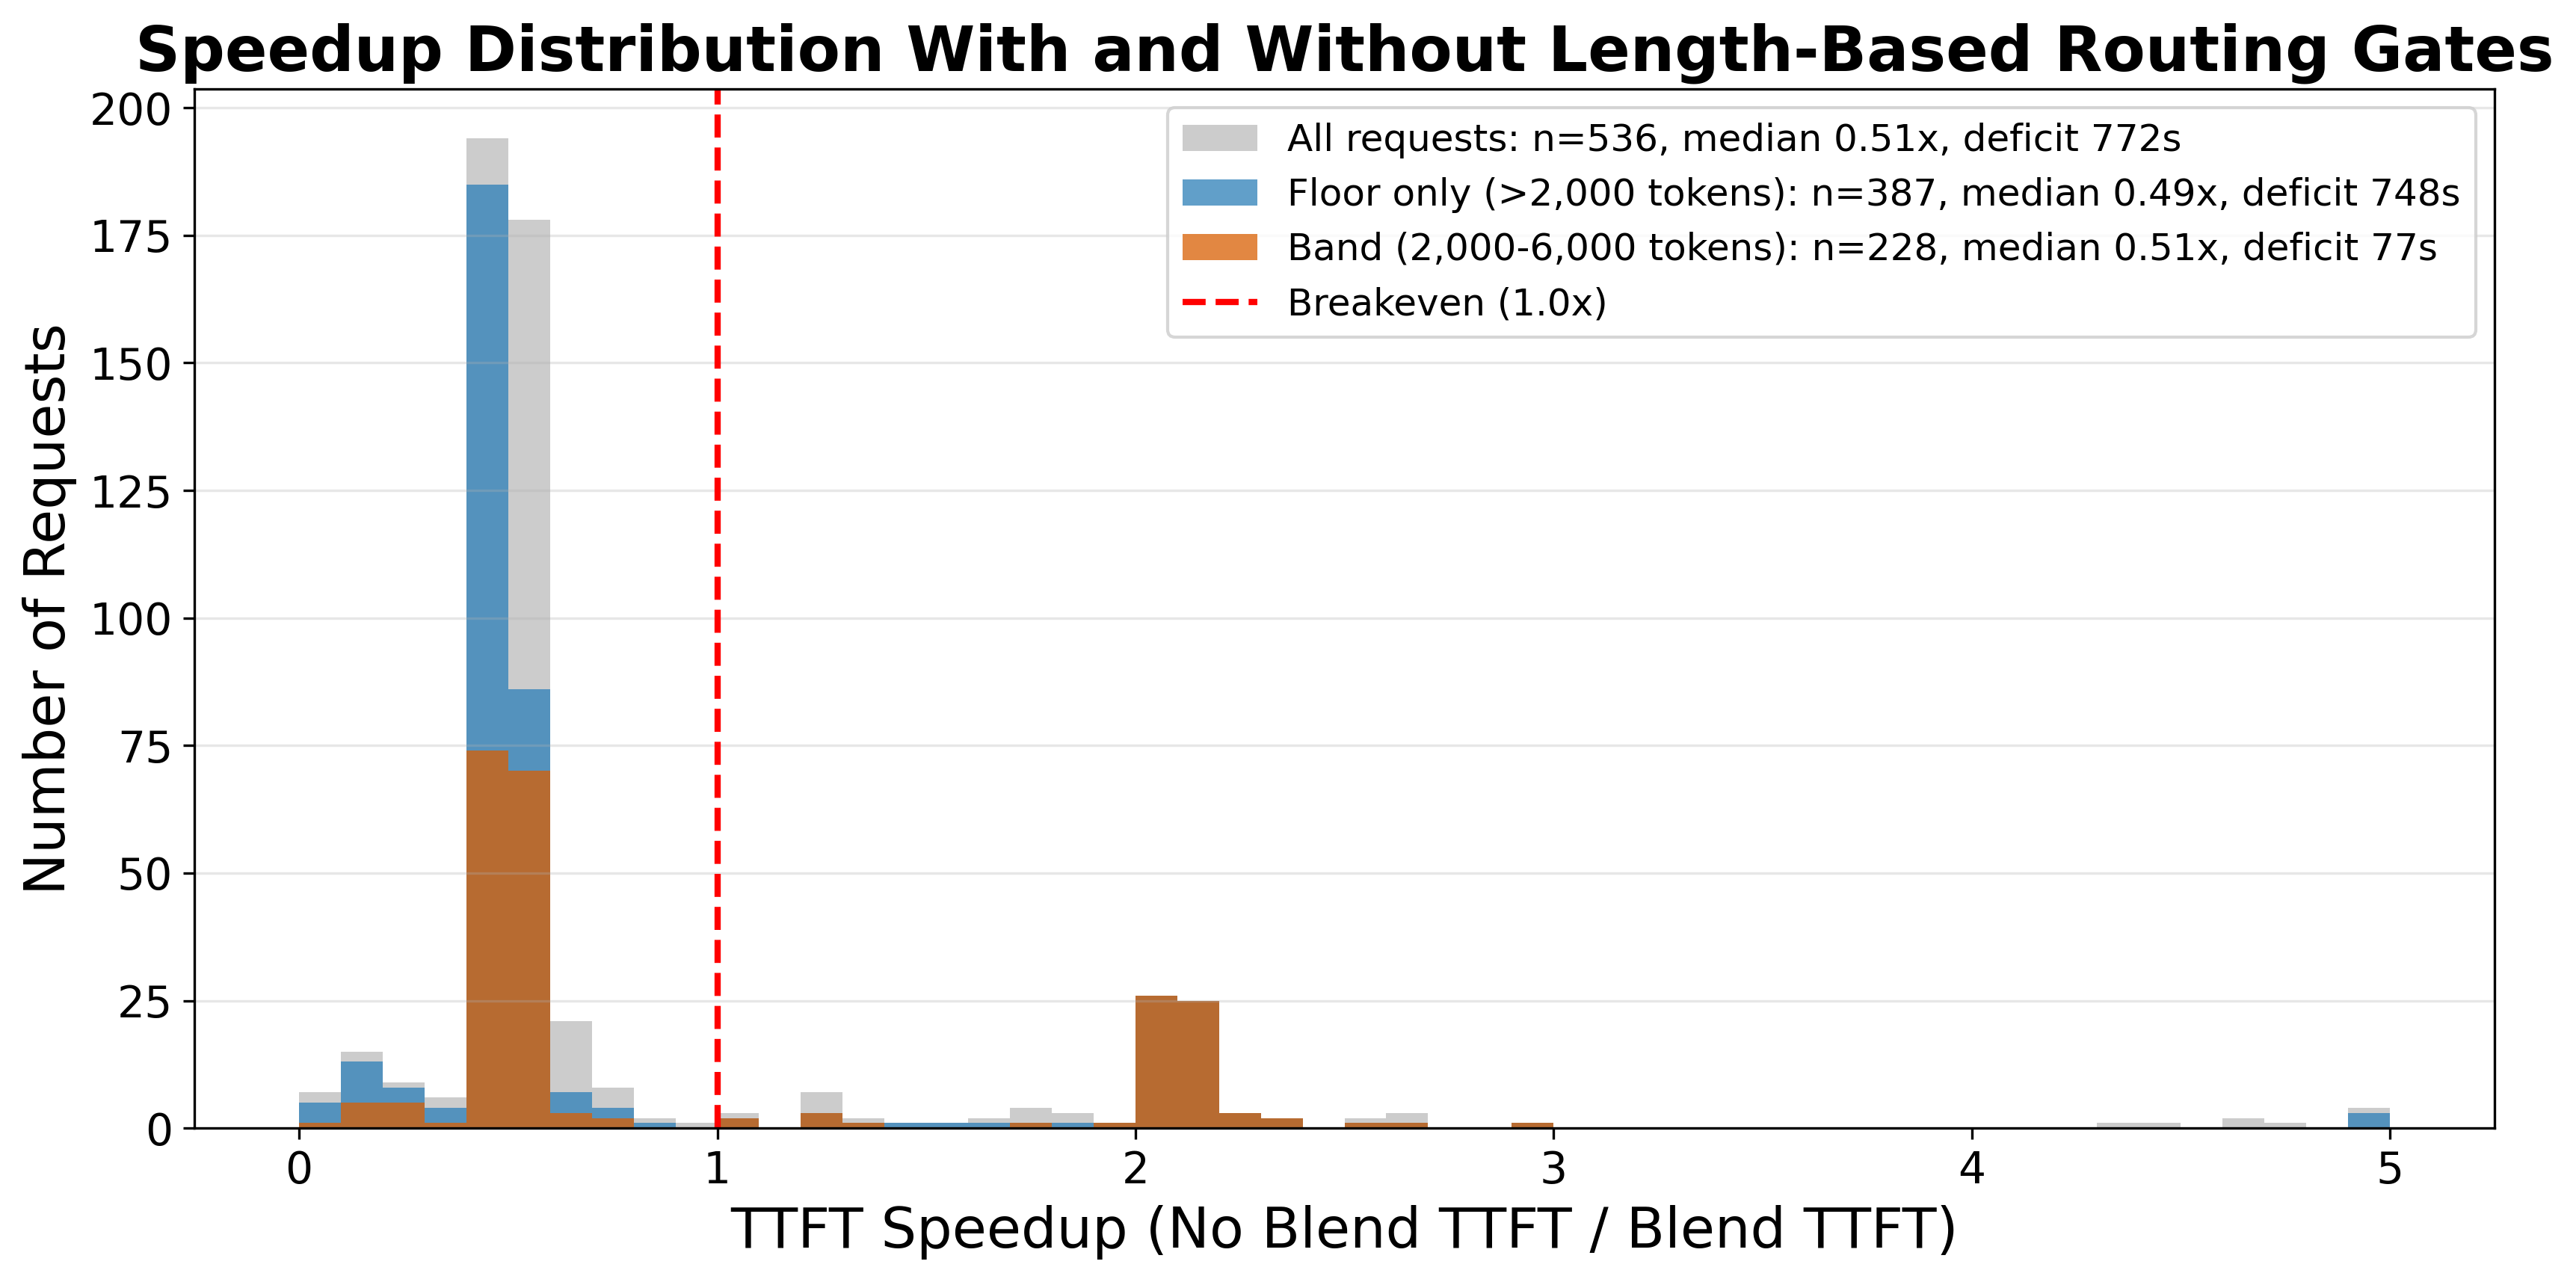
\includegraphics[width=0.9\linewidth]{graphs/thesis_variance_figures/speedup_histogram_length_gated.png}
\vspace{-0.1in}
  \caption{\small Per-request TTFT speedup under three routing policies. Bypassed requests are served by vanilla vLLM and sit at exactly 1.0$\times$ by construction, so they are excluded and each histogram shows only the requests still taking the cache path. The legend reports the aggregate deficit for each policy.}
 \label{fig:gated_hist}
 \vspace{-0.15in}
\end{figure}

Figure~\ref{fig:gated_hitratio} shows the same policy in the coordinates of Figure~\ref{fig:speedup_3d}, with the prompt-length dimension dropped so that only the routing decision is visible. The band retains 228 of the 532 plotted requests, including 68 of the 105 well-cached ones, and its routed set has a median speedup of 0.509$\times$, essentially unchanged from the ungated trace. The figure shows why both facts hold at once. Routed and bypassed requests appear in both hit-ratio clusters, so the band does not sort requests by whether they will hit. What it does instead is remove the long prompts, which are the requests whose misses cost the most in absolute terms. That is enough to recover most of the aggregate deficit without moving the per-request distribution, and it is the sense in which prompt length is a useful routing signal here.

\begin{figure}[H]
\centering
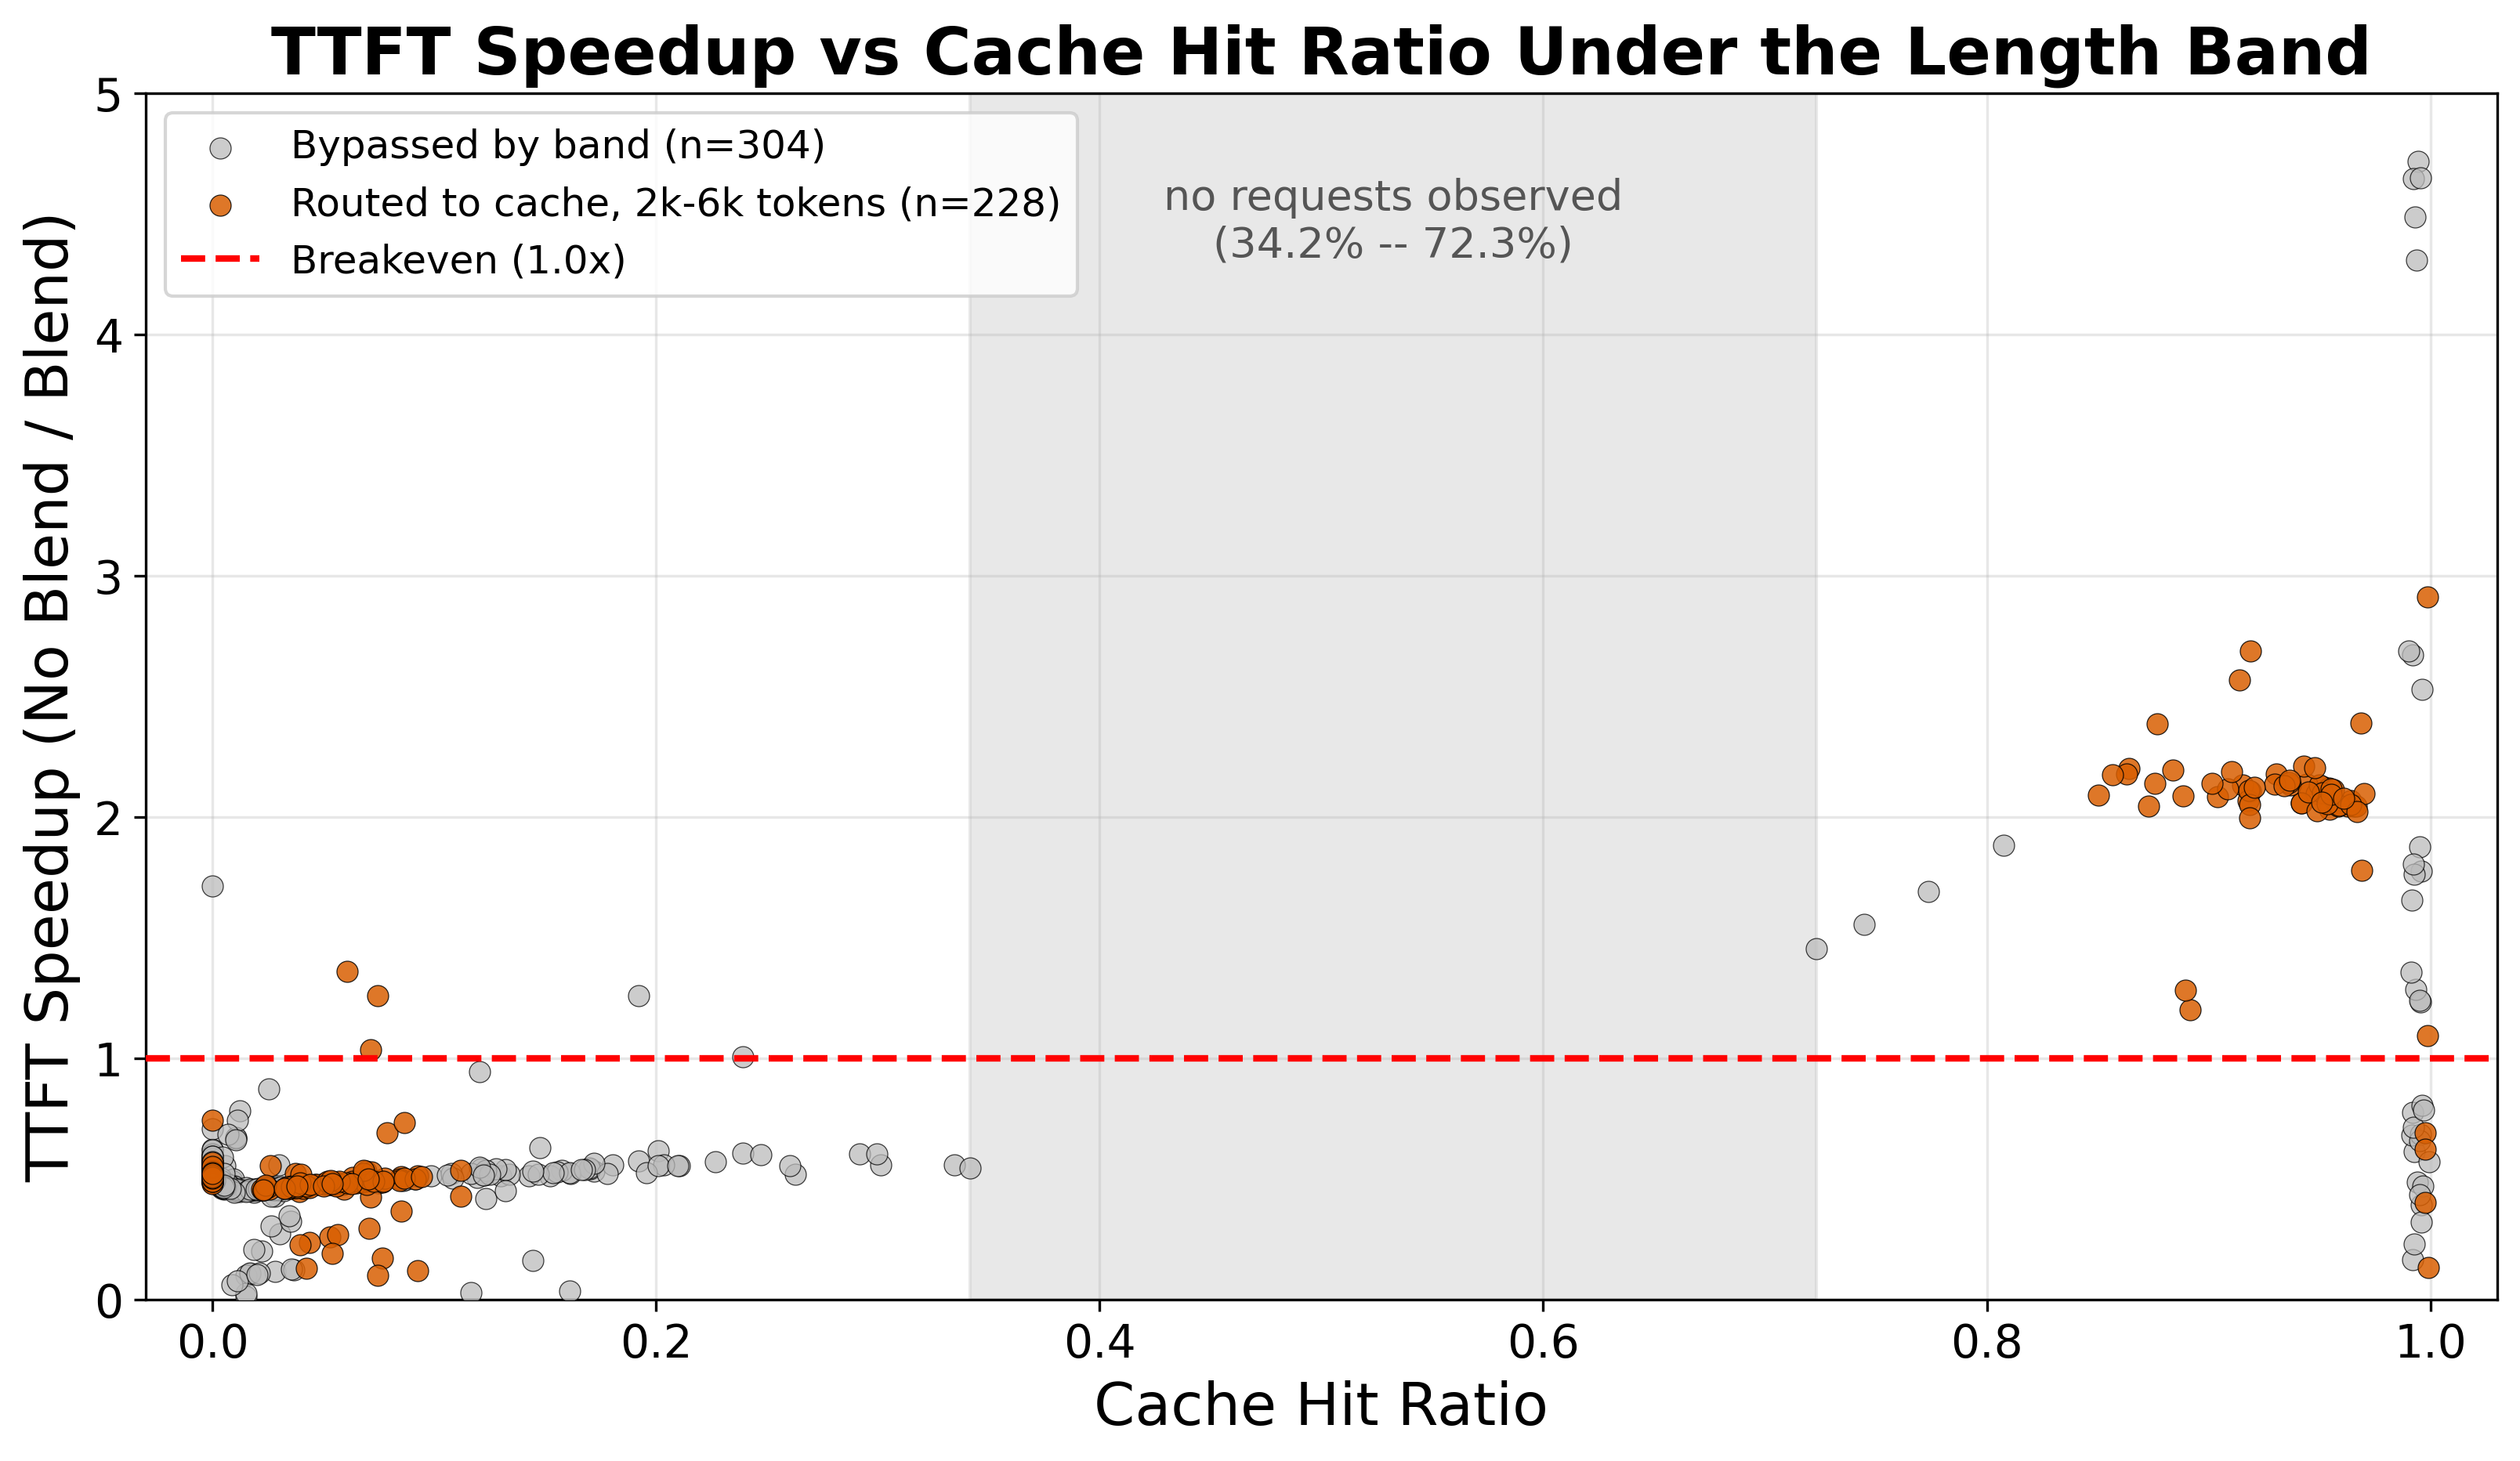
\includegraphics[width=0.9\linewidth]{graphs/thesis_variance_figures/speedup_vs_hitratio_gated.png}
\vspace{-0.1in}
  \caption{\small TTFT speedup against cache hit ratio under the 2{,}000 to 6{,}000 token routing band, using the colours of Figure~\ref{fig:gated_hist}. Orange points are routed to the cache, grey points bypass it. The band admits many low-hit requests and turns away well-cached ones, because prompt length separates the two clusters only weakly.}
 \label{fig:gated_hitratio}
 \vspace{-0.15in}
\end{figure}

\rashmi{Add a plot which shows only the allowed band (i.e., after removing very small and very long requests) visualzing the cache hit ratio. }

\subsubsection{Proposed Controller}
\label{sec:rec_controller}

Taken together, these results argue for treating the LMCache layer as optional per request, mediated by a controller in front of the backend that applies two independent rules.

The first is a length band rather than a floor. Prompt length is known before dispatch, so the rule is cheap to evaluate, and the upper threshold is where nearly all of its value lies. The floor contributes little on its own and is best justified as protection against the short requests that cannot win even when they hit.

The second rule concerns reuse, and it is the one that determines whether the system is profitable overall. Since the outcome is governed by whether a request will hit, the controller needs an estimate of hit likelihood before it commits to the cache path. Both rules govern only \emph{whether} a request takes the cache path, never what the model receives, so neither can affect the quality of the generated patch. Section~\ref{sec:ch1_eval} verifies the corresponding property of the cache path itself: that reusing KV state across positions leaves output quality intact.

\subsubsection{Next Steps}
\label{sec:rec_next_steps}

Three concrete steps follow from this case study, in decreasing order of expected value.

\emph{Move the KV store off the critical path.} Section~\ref{sec:rec_miss_penalty} attributes the roughly 2$\times$ miss penalty to the synchronous offload, which the roughly 80\% of requests that miss pay in full. Making the offload asynchronous would remove that penalty without changing the reuse mechanism at all, and would make the routing question far less pressing.

\emph{Build and validate a reuse predictor.} A cheap approximation is available in the agentic setting: the frontend knows which context objects it assembled into the prompt, so it can report how many of them it has already sent. That estimate can be attached to the request and used to route. Validating it requires a trace that samples hit ratio continuously, which ours does not, as noted in Section~\ref{sec:conclusion_future}.

\emph{Deploy the length band as an interim measure.} Until the store path is asynchronous and a predictor exists, an upper threshold near 6{,}000 tokens recovers most of what length-based routing can recover on this workload. A deployment that cannot predict reuse at all is better served by enabling LMCache selectively, for workloads known to have high context overlap, rather than by default.

